\documentclass{article}

\usepackage[final]{style}
\usepackage[utf8]{inputenc} % allow utf-8 input
\usepackage[T1]{fontenc}    % use 8-bit T1 fonts
\usepackage{hyperref}       % hyperlinks
\usepackage{url}            % simple URL typesetting
\usepackage{booktabs}       % professional-quality tables
\usepackage{amsfonts}       % blackboard math symbols
\usepackage{nicefrac}       % compact symbols for 1/2, etc.
\usepackage{microtype}      % microtypography
\usepackage{verbatim}
\usepackage{graphicx}       % for figures

\usepackage{caption}
\usepackage{graphicx, subfig}

\usepackage{amsmath,bm}

\usepackage{mathrsfs}
\usepackage{amssymb}

% Self-defined macros
\newcommand{\matr}[1]{\mathbf{#1}}
\newcommand{\proba}[1]{\mathsf{P}(#1)}
\newcommand{\expect}[1]{\mathsf{E}[#1]}
\newcommand{\var}[1]{\mathsf{Var}(#1)}
\newcommand\defeq{\stackrel{\text{!}}{=}}

\title{Exercise 06 of Machine Learning [IN 2064]}

\author{
  Name: Yiman Li \\
  \textbf{Matr-Nr: 03724352} \\
  cooperate with Kejia Chen(03729686)\\
}

\begin{document}

\maketitle

\section*{Problem 1}
a) We can not figure out clearly the convexity of the function $h(\bm{x})$ here. \\
Take $n=1$ for instance. The second derivative of the composition function $h(\bm{x})$ is given by
\begin{equation}
h''(\bm{x}) = g_2''(g_1(\bm{x}))g_1'(\bm{x})^2 + g_2'(g_1(\bm{x}))g_1''(\bm{x})
\end{equation}
Since we don't know whether $g'_2(x)$ positive or negetive is, so the symbol of $h''(x)$ is ambigious, so we can not safely say that $h(\bm{x})$ here is convex.\\

b) We can prove that $h(\bm{x}) = g_2(g_1(\bm{x}))$ is convex in the given condition. \\
According to the book \cite{Boyd:2004:CO:993483}, firstly 
\begin{itemize}
	\item Since $g_1(\bm{x})$ is convex, so $g_1''(\bm{x}) \geq 0$;
	\item Since $g_2(\bm{x})$ is convex and non-decreasing, so $g''_2(\bm{x}) \geq 0 $ and $g'_2(\bm{x}) \geq 0$.
\end{itemize}
The second derivative of the composition function $h(\bm{x})$ is given by
\begin{equation}
	h''(\bm{x}) = g_2''(g_1(\bm{x}))g_1'(\bm{x})^2 + g_2'(g_1(\bm{x}))g_1''(\bm{x}) \geq 0
\end{equation}
i.e., $h(\bm{x}) = g_2(g_1(\bm{x}))$ is convex.\\

c) We can prove that $h(\bm{x})$ is convex if $\bm{\mathrm{dom}}\ h = \bm{\mathrm{dom}}\ g_1 \bigcap \bm{\mathrm{dom}}\ g_2 \bigcap \dots \bigcap \bm{\mathrm{dom}}\ g_n$. \\
First we consider that $h_2(\bm{x}) = \max (g_1(\bm{x}), g_2(\bm{x}))$,  then we can derive that
\begin{equation}
	\begin{aligned}
		h_2(\theta x + (1-\theta)y)
		&= \max \{g_1(\theta x + (1-\theta)y), g_2(\theta x + (1-\theta)y)\}\\
		&\leq \max \{\theta g_1(x) +(1-\theta)g_1(y), \theta g_2(x) +(1-\theta)g_2(y)\}\\
		&\leq \theta \max\{g_1(x), g_2(x)\} + (1-\theta)\max\{g_1(y), g_2(y)\}\\
		&= \theta h_2(x) + (1-\theta)h_2(y)
	\end{aligned}
	\label{primitive function}
\end{equation}
The equations above establish the convexity of $h_2(\bm{x})$. Then  using the recursive method, we first assuming that $h_{n-1}(\bm{x}) = \max (g_1(\bm{x}), g_2(\bm{x}), \dots, g_{n-1}(\bm{x}))$ is a convex, then
\begin{equation}
	\begin{aligned}
		h(\theta x + (1-\theta)y)
		&= \max \{h_{n-1}(\theta x + (1-\theta)y), g_n(\theta x + (1-\theta)y)\}\\
		&\leq \max \{\theta h_{n-1}(x) +(1-\theta)h_{n-1}(y), \theta g_n(x) +(1-\theta)g_n(y)\}\\
		&\leq \theta \max\{h_{n-1}(x), g_n(x)\} + (1-\theta)\max\{h_{n-1}(y), g_n(y)\}\\
		&= \theta h(x) + (1-\theta)h(y)
	\end{aligned}
	\label{further function}
\end{equation}
Combining equation \ref{primitive function} and equation \ref{further function}, we can say that $h(\bm{x}) = \max (g_1(\bm{x}), g_2(\bm{x}), \dots, g_n(\bm{x}))$ is also convex.

\section*{Problem 2}
a) The objective function can be rewritten as
\begin{equation}
	\begin{aligned}
		f(x_1, x_2)
		&= 0.5x_1^2 + x_2^2 + 2x_1 + x_2 + \cos(\sin(\sqrt{\pi}))\\
		&= 0.5(x_1^2 + 4x_1 + 4) + (x_2^2 + x_2 + \frac{1}{4}) + \cos(\sin(\sqrt{\pi})) - \frac{9}{4}\\
		&= 0.5(x_1 + 2)^2 + (x_2 + \frac{1}{2})^2 + \cos(\sin(\sqrt{\pi})) - \frac{9}{4}\\
		&\geq \cos(\sin(\sqrt{\pi})) - \frac{9}{4}
	\end{aligned}
\end{equation}
The equality is reached when $\bm{x}^* = (-2, -\frac{1}{2})^T$.

b) The derivative of the function can be written as
\begin{equation}
	f'(x_1,x_2) = (x_1+2, 2x_2+1)
\end{equation}
starting from $\bm{x}^{(0)}$ and $\tau=1$, we have
\begin{equation}
	\begin{aligned}
		\bm{x}^{(1)} &= \bm{x}^{(0)} - \tau \cdot f_0'(x_1,x_2) = (0,0)-(2,1) = (-2, -1)\\
		\bm{x}^{(2)} &= \bm{x}^{(1)} - \tau \cdot f_1'(x_1,x_2) = (-2,-1)-(0,-1) = (-2, 0)\\
		\bm{x}^{(3)} &= \bm{x}^{(2)} - \tau \cdot f_2'(x_1,x_2) = (-2,0)-(0,1) = (-2, -1)	
	\end{aligned}
\end{equation}

c) Oberseving from $\bm{x}^{(1)}$, $\bm{x}^{(2)}$ and $\bm{x}^{(3)}$, we can see that the function has run into an infinite loop and it can never converge to the true minumum $\bm{x}^*$ due to the oscillations resulted from too large learning rate. On this condition we should tune our learning rate a bit more smaller. But attention should be paid to other problems, for examply, we may find the minimum slowly, or end up in local minima or saddle points.

\section*{Problem 3}
Show in the end.

\section*{Problem 4}
a) No! the shaded region $S$ in $\mathbb{R}^2$ is not convex. As shown in Figure \ref{not convex proof},
\begin{figure}[htbp]
	\centering
	\begin{minipage}{5cm}
		\centering
		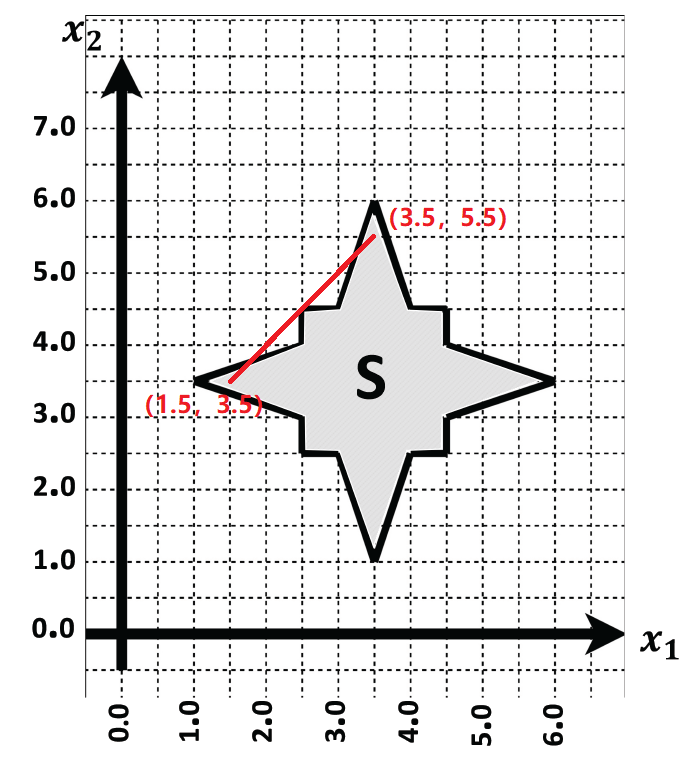
\includegraphics[scale=0.5]{not_convex.png}
		\caption{Not a convex}
		\label{not convex proof}
	\end{minipage}
	\begin{minipage}{5cm}
		\centering
		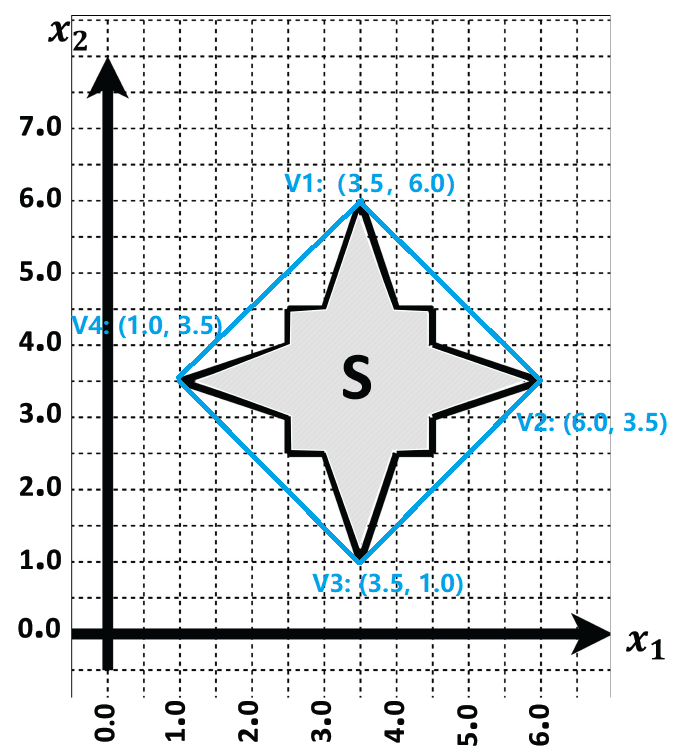
\includegraphics[scale=0.5]{find_maximum.png}
		\caption{Convex after filling}
		\label{find the maximum}
	\end{minipage}		
\end{figure}
we draw a line between the two points $(1.5,3.5)$ and $(3.5, 5.5)$, and there exist some points on the line distributed outside of the shaded region. That is to say, not all the point follows the law that
\begin{equation}
	\lambda x + (1-\lambda)y \in X\ \ \mathrm{for}\ \lambda \in [0,1]
\end{equation}
So the region here is not convex.

b) Since the maximum over a convex function on a convex set is obtained on a vertex, so as shown in Figure \ref{find the maximum}, we simply connecting four vertices, namely, $V_1(3.5, 6.0)$, $V_2(6.0, 3.5)$, $V_3(3.5, 1.0)$, $V_4(1.0, 3.5)$ of the shaded region, and now the augumented region becomes convex. So the maximum of convex function $f(x_1, x_2) = e^{x_1+x_2} - 5\mathrm{log}(x_2)$ must be one of these four vertices, so just compute:
\begin{equation}
	\begin{aligned}
		f_{V_1}(x_1, x_2) &= f(3.5, 6.0) = e^{9.5} - 5\mathrm{log}(6.0) = 13346.80\\
		f_{V_2}(x_1, x_2) &= f(6.0, 3.5) = e^{9.5} - 5\mathrm{log}(3.5) = 13350.69\\
		f_{V_3}(x_1, x_2) &= f(3.5, 1.0) = e^{4.5} - 5\mathrm{log}(1.0) = 90.02\\
		f_{V_2}(x_1, x_2) &= f(1.0, 3.5) = e^{4.5} - 5\mathrm{log}(3.5) = 80.98
	\end{aligned}
\end{equation}
So the maximum of $f$ over the shaded region $S$ is obtained at the point $\bm{x}^* = (6.0, 3.5)$.

c) We can divide the shaded region into the combination of five sub-region, as is shown in Figure \ref{find the minimum}, namely, $S = S_1 \bigcap S_2 \bigcap S_3 \bigcap S_4 \bigcap S_5$, with every sub-region being convex region. Then we can use the algorith ConvOpt$(f, D)$ to find the minimum on every sub-region. At last, we need to make contrast among these local minimums, and finally find the true global minimum.
\begin{figure}
	\centering
	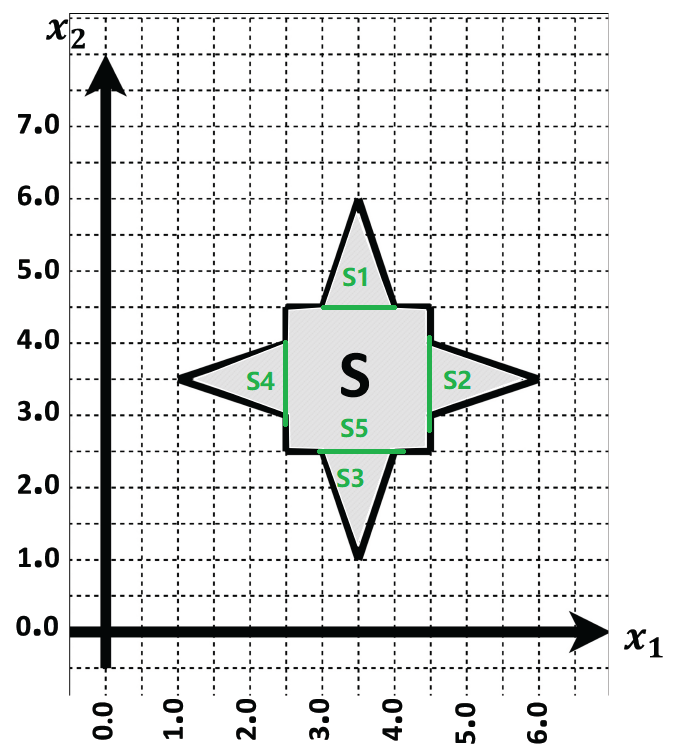
\includegraphics[scale=0.5]{region_distribution.png}
	\caption{Five sub-region}
	\label{find the minimum}
\end{figure}


% References
\small
\bibliographystyle{plain}
\bibliography{bibliography6}
\end{document}
